\section{Measurement and Evaluation}
\subsection{Characteristics of the CCD and data reduction}
We visualize and analysis the data image using \textit{Python} with the packages \textit{astropy}, \textit{ccdproc}, \textit{numpy} and \textit{matplotlib} and the image display program \textit{ds9} to check the .fits images produced by the CCD detector and the \textit{python scripts}.
\subsubsection{Bias correction}
As explained in section \ref{reduction}, we first determine the bias from the overscan region on the right edge of CCD images of dark measurements. We then subtract said bias from the whole image to get a bias free image. We determine the overscan region to be in the are x $>$ 1024 for all y with \textit{ds9}. In figure \ref{darks} you can see 3 different measurements with shutter closed and bias subtracted. We can clearly see the overscan region as long as you have a signal. The bias of the uncorrected first image in figure \ref{13th} is $1374.0 \pm 5.2$, of the second image in figure \ref{70th}  $1334.0 \pm 1.8$ and of the last image in figure \ref{174th} $1350.0 \pm 1.7$. \\
\begin{figure}[h]
	\begin{subfigure}{0.32\textwidth}
	\centering
	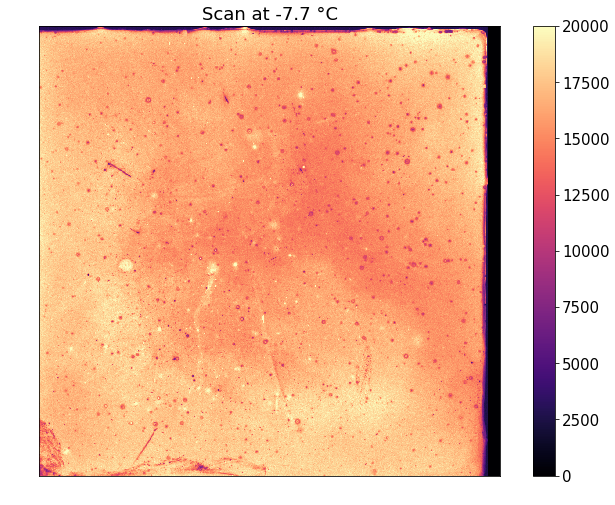
\includegraphics[width=0.95\linewidth]{report_pictures/s12.png}
	\caption{13th image}
	\label{13th}
	\end{subfigure}
	\begin{subfigure}{0.32\textwidth}
	\centering
	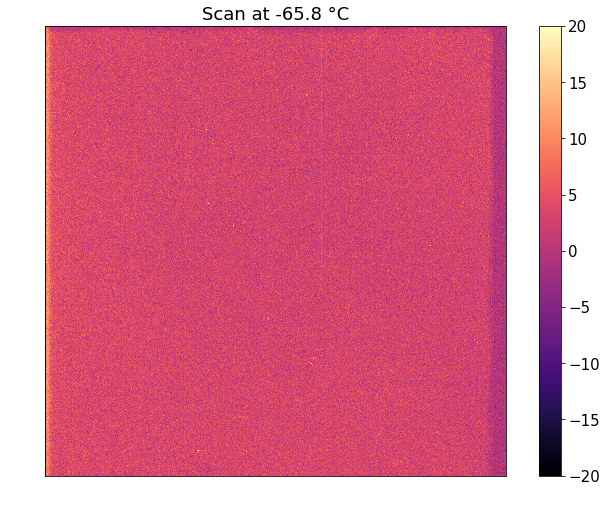
\includegraphics[width=0.95\linewidth]{report_pictures/s70.png}
	\caption{70th image}
	\label{70th}
	\end{subfigure}
	\begin{subfigure}{0.32\textwidth}
	\centering
	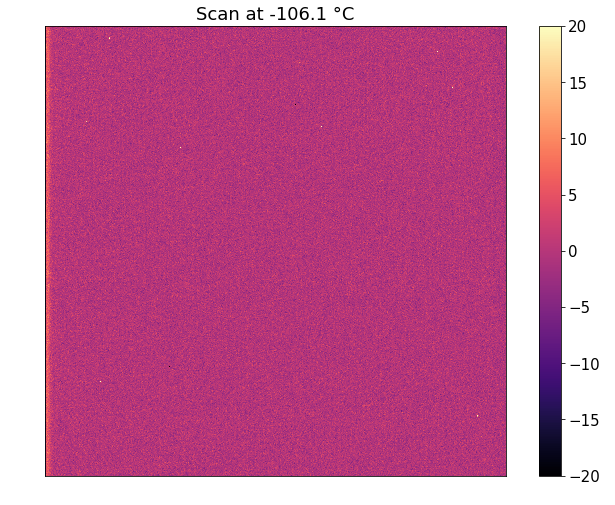
\includegraphics[width=0.95\linewidth]{report_pictures/s173.png}
	\caption{174th image}
	\label{174th}
	\end{subfigure}
	\caption{Dark current measurements at different Temperatures}
	\label{darks}
\end{figure} 

\subsubsection{Dark measurements}
From the bias subtracted pictures we can now extract the dark current by calculating the median of each picture. By plotting \textit{counts}$T^{-\frac{3}{2}}$ over $T^{-1}$ on a log scale seen in figure \ref{band_gap_fit} we can determine the band gap by fitting an equation to the data set. To get the fit function we rearrange eq \eqref{dark_current} to match the quantities we have plotted. This gives a function as follows:
\begin{equation}
\label{Eg}
	\textit{counts }T^{-\frac{3}{2}} = \textit{const }e^{-\frac{E_g}{2k_BT}}
\end{equation}
\begin{figure}[h]
	\centering
	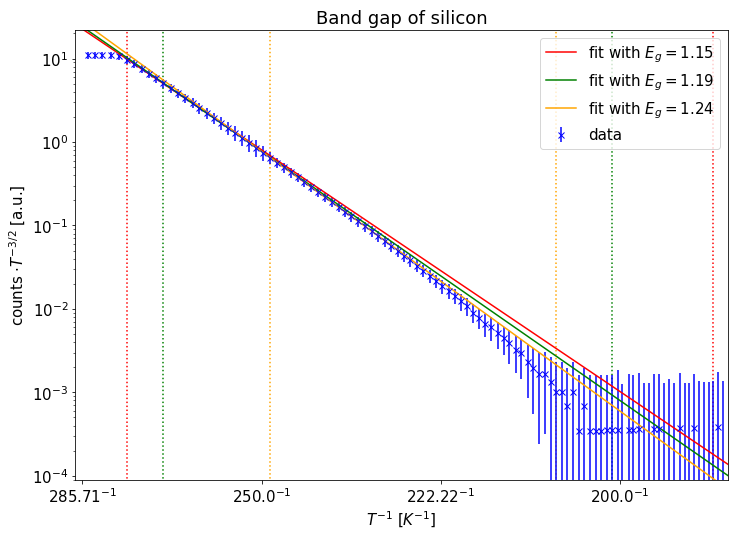
\includegraphics[width=0.9\textwidth]{report_pictures/BandGap.png}
	\caption{Data of the dark current measurement plotted and fitted}
	\label{band_gap_fit}
\end{figure}
where Boltzmann constant $k_B = 8.617 \cdot 10^{-5} \frac{eV}{K}$ and $E_g$ is the band gap of silicone.  We now fit a function on that data set and determine $E_g$ from on the 2 parameters. We fit with 3 different fit ranges, indicated by the different coloured dotted lines to approximate an error with those fits. We do this since the approximation seems to deviate a lot for lower temperatures, but still results in a small error in the range 2 - 3 \textit{meV}. This can be explained by remembering that this is a log scale, meaning the values on the bottom right of the fit are several magnitudes smaller then the values that seem to be right on the fit in the top left. Hence we use the fit range variation to approximate an error for our measurement which leads us to a value of $E_g = 1.19 \pm 0.4$ \textit{eV}. The literature value is given as $1.15$ eV. This $1\sigma$ deviation as well as the overall deviation of the fit for lower temperatures can be explained by two main reasons. \\
First, the temperature is only measured once at the start of the exposure time, with no further information saved about the change over the exposure time. Also the temperature has no error associated with it since we didn't average over several measurements nor did we have any information on the precision of the sensor.\\
Second, the band gap is not constant for different Temperature. It has a dependency on T which can be described \cite{band_gap_dep} as follows:
\begin{equation}
	\label{band_gap_depen}
	E_g = E_{g,0} - \dfrac{\alpha T^2}{T + \beta}
\end{equation}
$\alpha$ and $\beta$ are material constants, T is the temperature and $E_{g,0}$ is the band gap at 0 K.\\ The second argument leads to a higher band gap for lower temperature, which is reflected in our data as well since the fit with the higher band gap is the ones which is more fitting for the lower temperatures.
\vspace{2mm}\\
Looking at the image in figure \ref{174th} we can conclude, that at our working temperature of roughly $-106 \degree C$ the dark current is indeed small enough to ignore. 
\vspace{4mm}
\subsubsection{Flat-field correction}
After subtracting the bias from the individual flat-field images, we combine the individual flat-field images to a single image (the master flat-field). We set all values below a certain threshold to 0 so those pixel get valued as NAN when evaluating images. Then we normalize the master flat-field by dividing it by its median and create a histogram for this master flat-field as shown in figure \ref{hist}. \\
\begin{wrapfigure}{l}{0.5\textwidth}
	\centering
	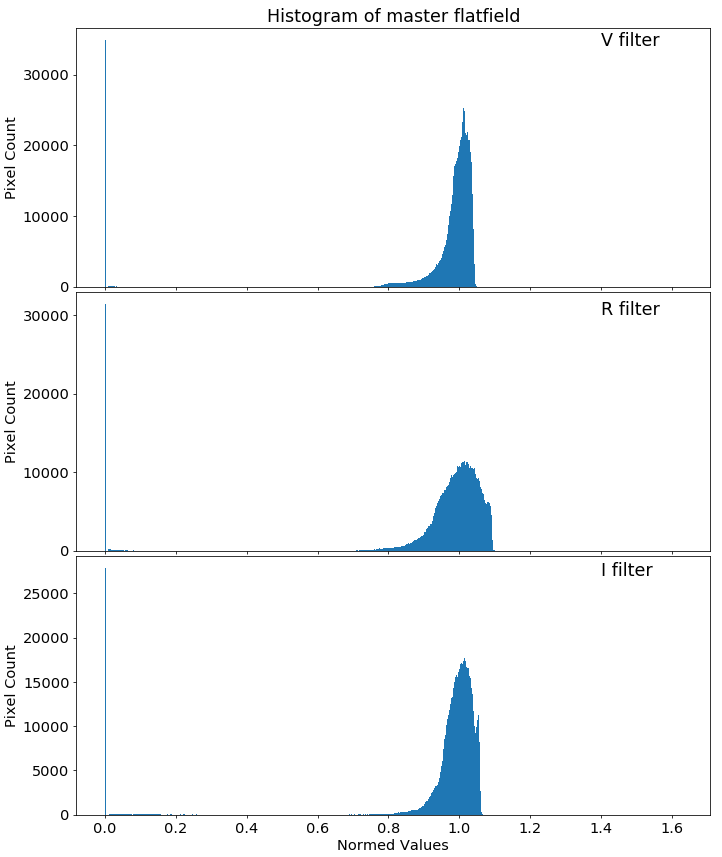
\includegraphics[width=0.45\textwidth, height=8cm]{report_pictures/FlatHist.png}
	\caption{Histograms of the normalized master flat-fields for the 3 filters of our CCD}
	\vspace{-10pt}
	\label{hist}
\end{wrapfigure}
The bar at 0 indicates the overscan region (which has 26624 pixels) as well as dead pixels or dead regions on filter through contaminations. Most of pixel group around the median value, i.e. 1 on the x-axis, though there are a lot more below 1 then above. This can be explained by realizing that the group below one has a lot a more sources than only the optical effects like \textit{vignette} effect which are the reason for the deviation above as well as under. The group under 1 contains all the optical containments from which not all result in a full photon block, rather they only reduce the photon amount.
\vspace{4mm}\\
To grasp what those effects could look like and how we compensate those, we perform a flat-field correction for a single flat-field image with the I filter and compare the uncorrected image with the corrected one. The comparison of two plots is shown in figure \ref{flat_ex}. One can see the symmetrical effects very clearly in \ref{flat_before} as well as the optical containments. After the correction seen in figure \ref{flat_after} we can see that the image has become \textit{flat}, i.e. evenly distributed, by changing its range from 6000 pixels to less then 350 pixels. The green area here shows NAN values, meaning we tried to divide by a zero of the master flat-field. The difference between the pixels can be attributed to the noise we discussed in section \ref{noise}. Though statistical noise seems to be not the only source since one can see some weird shape in the image which seems to be not statistical nature. 
\vspace{4mm}\\
\begin{figure}[h]
	\begin{subfigure}{0.45\textwidth}
	\centering
	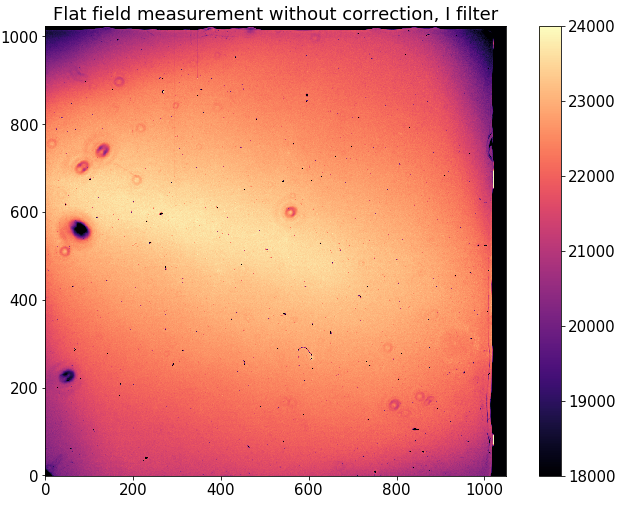
\includegraphics[width=0.95\linewidth]{report_pictures/FlatIFits.png}
	\caption{Image of the flat surface}
	\label{flat_before}
	\end{subfigure}
	\begin{subfigure}{0.45\textwidth}
	\centering
	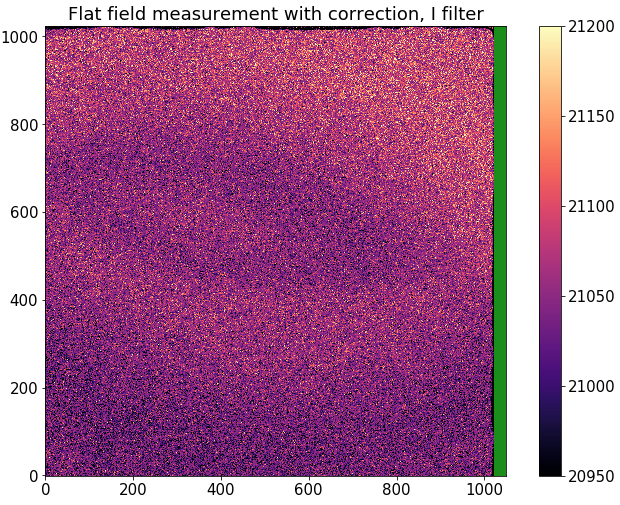
\includegraphics[width=0.95\linewidth]{report_pictures/FlatIFitsMasterCorrected.png}
	\caption{Flat-field corrected image}
	\label{flat_after}
	\end{subfigure}
	\caption{Example of an image getting corrected with the master flat-field}
	\label{flat_ex}
\end{figure} 
\subsubsection{Linearity and saturation area}
To verify the linearity as well as the saturation value of the chip, we plot the signal of each flat-field-corrected image against its exposure time. We do this for two different filters, I and R, where we just take one image of the pairs taken with the I filter. To determine the deviation from a perfect linear relationship we calculated  $R^2$, which is closer 1 the better the linear dependence is, its exact formula can be found at \cite{rsq}. We calculate it for both linear fits and determine the saturation area with data from both measurements. The data and fits are shown in figure \ref{lin}.
\begin{figure}[h]
	\centering
	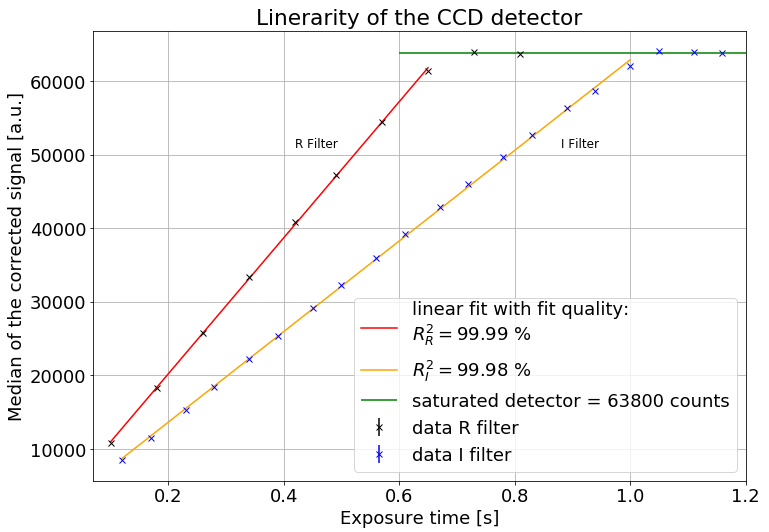
\includegraphics[width=0.8\textwidth]{report_pictures/Linearity.png}
	\caption{Verifying the linearity in 2 filters and determining the saturation area}
	\label{lin}
\end{figure}
\vspace{2mm}\\
Both filters show an exceptionally good $R^2$, deviating less than 0.02\% from the linear approximation. The saturated area can get determined to around 63800, meaning we should not exceed the 60000 counts if we wish to guarantee the linear characteristic from the CCD detector. Lastly we also see the dynamical range of the detector, since the filters take saturated at different exposure times which is a consequence of the spectrum of our light source (in our case the lamp illuminating our flat surface). 
\vspace{4mm}
\subsubsection{Sensitivity and noise}
\begin{wrapfigure}{r}{0.3\textwidth}
	\centering
	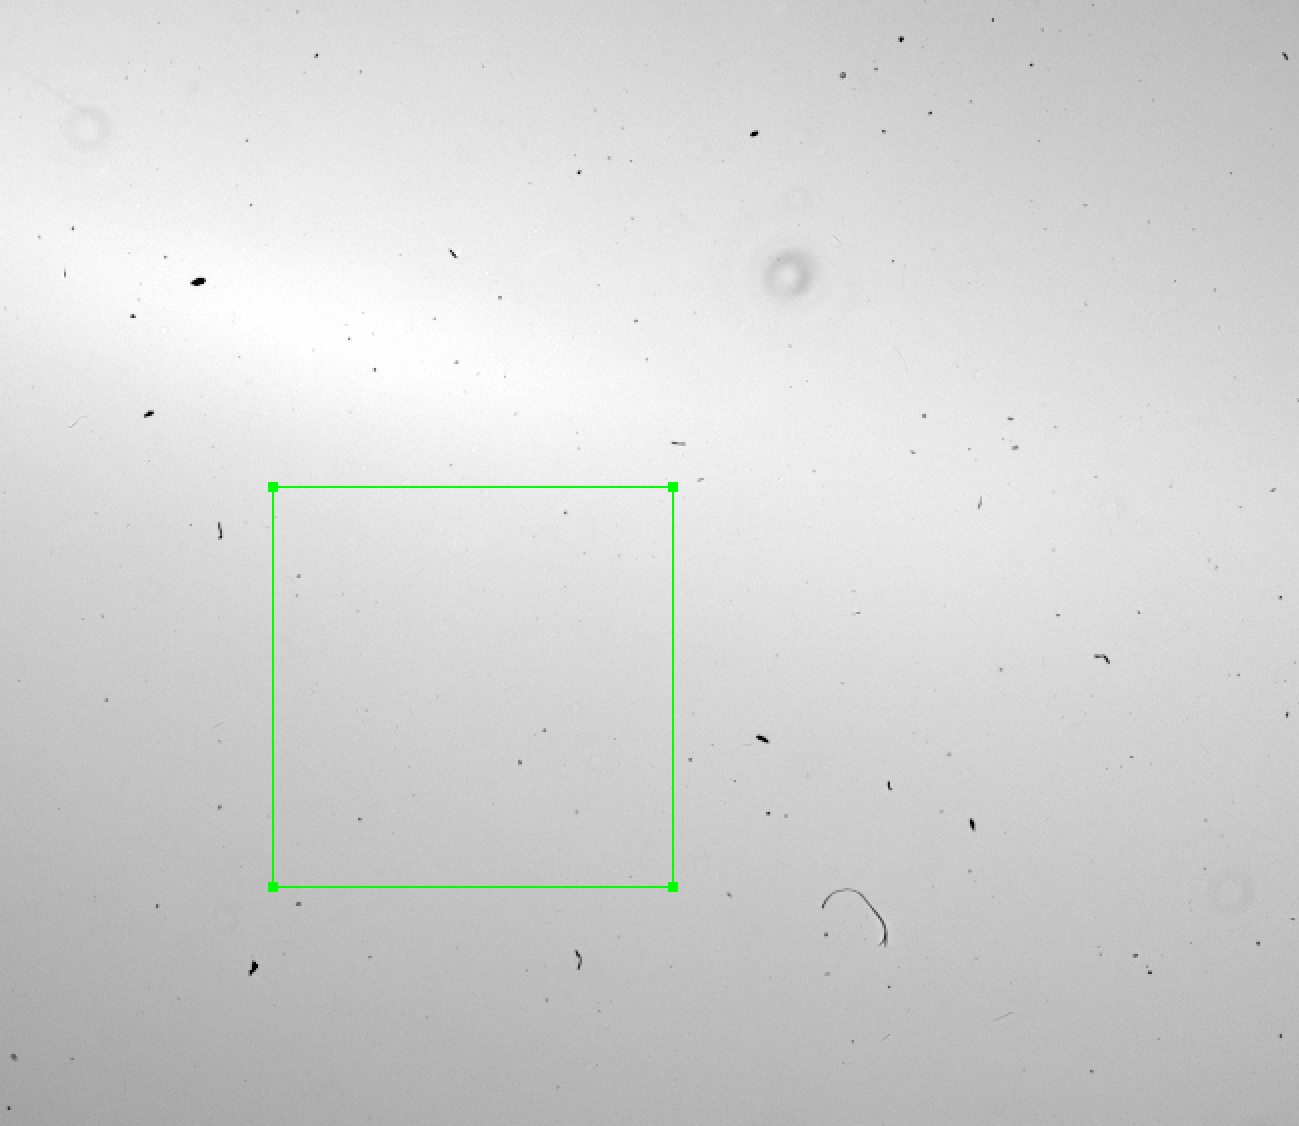
\includegraphics[width=0.25\textwidth, height=4cm]{report_pictures/sensitivity_region.png}
	\caption{Region for Noise}
	\vspace{-10pt}
	\label{area}
\end{wrapfigure}
To analyse the noise and calculate the gain with it we first chose an image pair with around 30000 counts and select a region around the middle which is as uniform as possible. That region is pictured in figure \ref{area}. First off we can calculate the read-out noise $\sigma_{r,d}$ by calculating the scatter in the overscan region. Second we calculate the total noise $\sigma_{tot,d}$ in that chosen area. We then continue to calculate the difference image of the chosen image pair and calculate the $\sigma_{diff,d}$ in the chosen region. We can then use eq \eqref{diff_img} and \eqref{sig_tot} to calculate $\sigma_{ph,d}$ and $\sigma_{prnu,d}$ shown in table \ref{errors1}.
\vspace{2mm}\\
As expected the $\sigma_ {prnu}$ dominates for high signal sources and the read-out noise is really small compared to the other noises caused by the independence on $N_{ph}$.
\begin{table}[h]
\centering
\begin{tabular}{c|c||c|c|c}
$\sigma_{tot,d}$ & $\sigma_{diff,d}$ & $\sigma_{rt,d}$ & $\sigma_{ph,d}$ & $\sigma_{prnu,d}$ \\
\hline
264.3 & 75.9 & 2.1 & 53.6 & 258.8 \\
\end{tabular}
\caption{Summery of the errors for an image with 30000 counts}
\label{errors1}
\end{table}
\vspace{12mm}\\
We can now calculate the gain from $\sigma_{ph,d}$ by using eq \ref{sig_phd} and approximating $\eta$ to be one. The gain gets calculated to $\kappa_1 = 10.85 \pm 0.03$ which is double the value we expected considering the \textit{header} of our fits say that the gain is 5. 
\vspace{3mm}\\
We can also calculate the gain differently. By inserting eq \ref{sig_phd} into eq \ref{diff_img} directly without calculating $\sigma_{ph,d}$, we get a linear dependency of $\sigma_{diff,d}^2$ on $N_{ph,d}$. If we now calculate the difference image of pairs with increasing median counts, i.e. increasing exposure time, we can plot the variance of these difference images versus the average of the median counts in the pair. This is shown in figure \ref{noise_diff}. 
\begin{figure}[h]
	\centering
	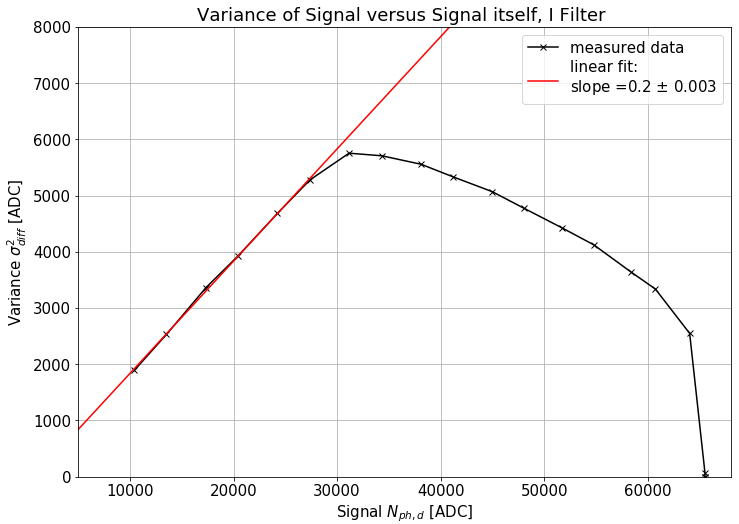
\includegraphics[width=0.8\textwidth]{report_pictures/Noise.png}
	\caption{Variance of the difference image versus the median counts of the images}
	\label{noise_diff}
\end{figure}
\vspace{2mm}\\
We can see that the linear dependency is very good till around 30000 counts, where it seems like other effects start to dominate which we didn't consider beforehand. Hence we will do the linear fit only till roughly 30000 counts to ensure the correctness of the fit. With that and the assumption of $\eta$ being one we can relate the slope to $\kappa$ by the double of its inverse $2\textit{slope}^{-1}$. This leads us to a gain of $kappa_2 = 10.02 \pm 0.13$. As already mentioned this is still double the value we expected, but this time it is exactly double the value.\\
\newpage
\subsection{CMD of globular cluster BS90}
We do most of the analysis for this part on a computer provided by the MPIA, which has \textit{STARFINDER} already installed as well as \textit{ds9} to view the pictures from the HST.
\subsubsection{PSF fitting}
To perform the PSF scan we first need \textit{STARFINDER} to determine the noise of both pictures. The noise histograms are shown in figure \ref{noise_star}. The dotted line is a Gaussian distribution fitted to the histogram to determine variance.
\begin{figure}[h]
	\begin{subfigure}{0.45\textwidth}
	\centering
	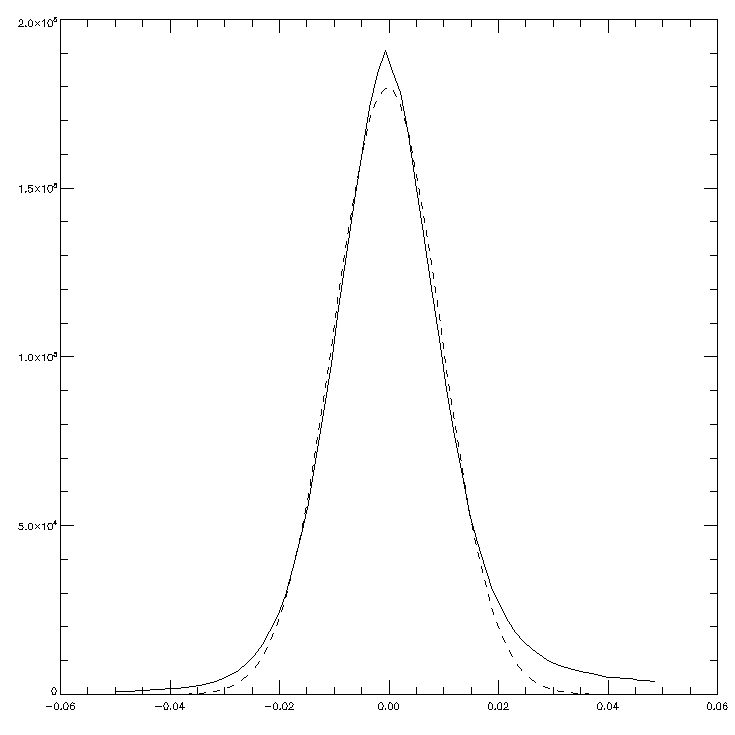
\includegraphics[width=0.95\linewidth]{report_pictures/NOISE_I_Histogram}
	\caption{I Filter Image}
	\label{noise_star_I}
	\end{subfigure}
	\begin{subfigure}{0.45\textwidth}
	\centering
	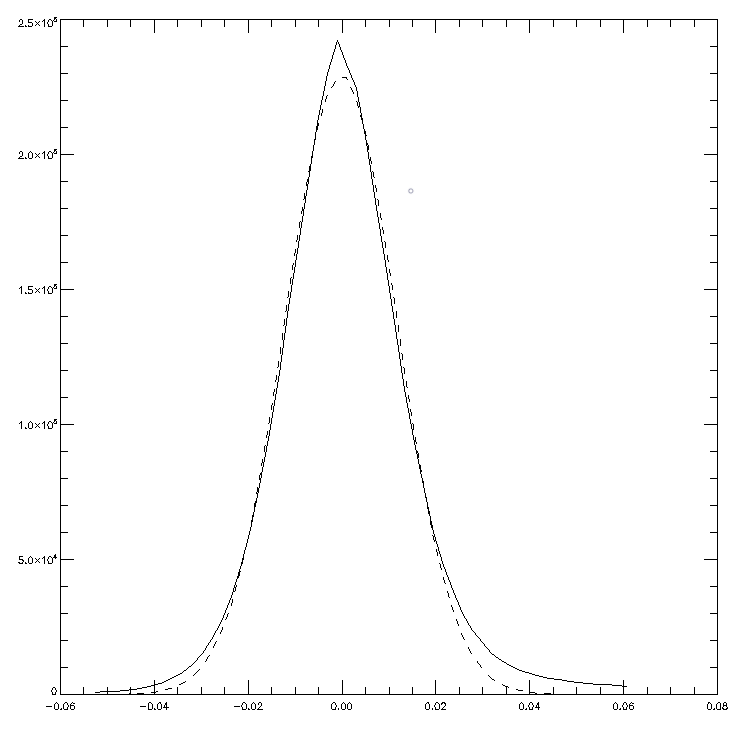
\includegraphics[width=0.95\linewidth]{report_pictures/NOISE_V_Histogram}
	\caption{V Filter image}
	\label{noise_star_V}
	\end{subfigure}
	\caption{Histogram of the noise on both filters, required to find stars}
	\label{noise_star}
\end{figure} 
\vspace{3mm}\\
After determining the noise we need to create a PSF so the program can search for the stars. We select 14 isolated, unsaturated stars. On a bounding box around the stars, an average PSF for the entire image is first created. Per editing we improve and optimize the PSF  by limiting its pixel range and normalizing it, as seen in figure \ref{PSF_post}. \\
\begin{wrapfigure}{l}{0.3\textwidth}
	\centering
	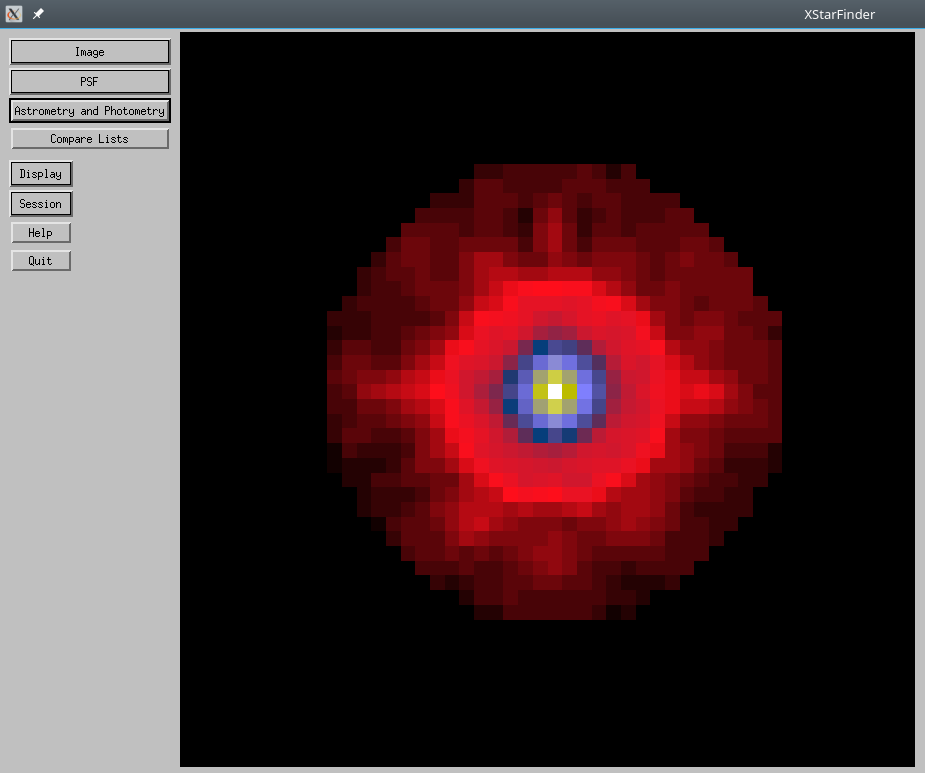
\includegraphics[width=0.28\textwidth ,height=4cm]{report_pictures/PSF_I_postprocessed.png}
	\caption{The post-processed PSF of the I filter}
	\label{PSF_post}
	\vspace{-15pt}
\end{wrapfigure}
Now we let the program determine all possible stars. All sources above a certain threshold above the background level are detected as potential stars. All potential stars are then fitted with the PSF and the results of this fitting is subtracted from the science image. This step is performed iteratively. That way we can disentangle and correctly account for the flux of overlapping sources.

\subsubsection{Zeropoint calibration}
Since the measurements were carried out with two filters a calibration is needed in order to compare their results. We overplot the HST images with data base \textit{SIMBAD}. We select 12 reference stars , which were calibrated themselves from true standard stars, write down the V and I magnitudes and measure their counts in both Hubble images. 
\vspace{2mm}
The instrumental magnitude is compared with the CATALOG objects to calculate the individual zero points for all objects for both filters according to formula:
\begin{equation}
\label{calibration}
	zeropoint = m_{CATALOG} + 2.5 \log_{10}{(counts)}
\end{equation}
We take the median as final zero point values, which gives us $zero_V = 25.15702$  and $zero_I = 25.14337$. The apparent magnitude of found stars by PSF fitting can then be calculated by eq \ref{instrumental} with the calibrated zero points. We then use the mentioned python script provided by our tutor, to match all stars as well as write down their apparent magnitudes V and I which get calculated with the zero points we updated in the python script. 
\vspace{3mm}\\
\subsubsection{Plot CMD and fit isochrones}
We plot V versus V-I of these stars and thus obtain the CMD of BS90. Then we plot a set of theoretical \textit{isochrones} in the CMD, using another given Python script in which we can change the fit parameters, i.e. age, metallicity and the shift, i.e. the distance modulus, in the V axis, which gives us the distance to the cluster. Our best fit is shown in figure \ref{cmd_1}. 
\begin{figure}[h]
	\centering
	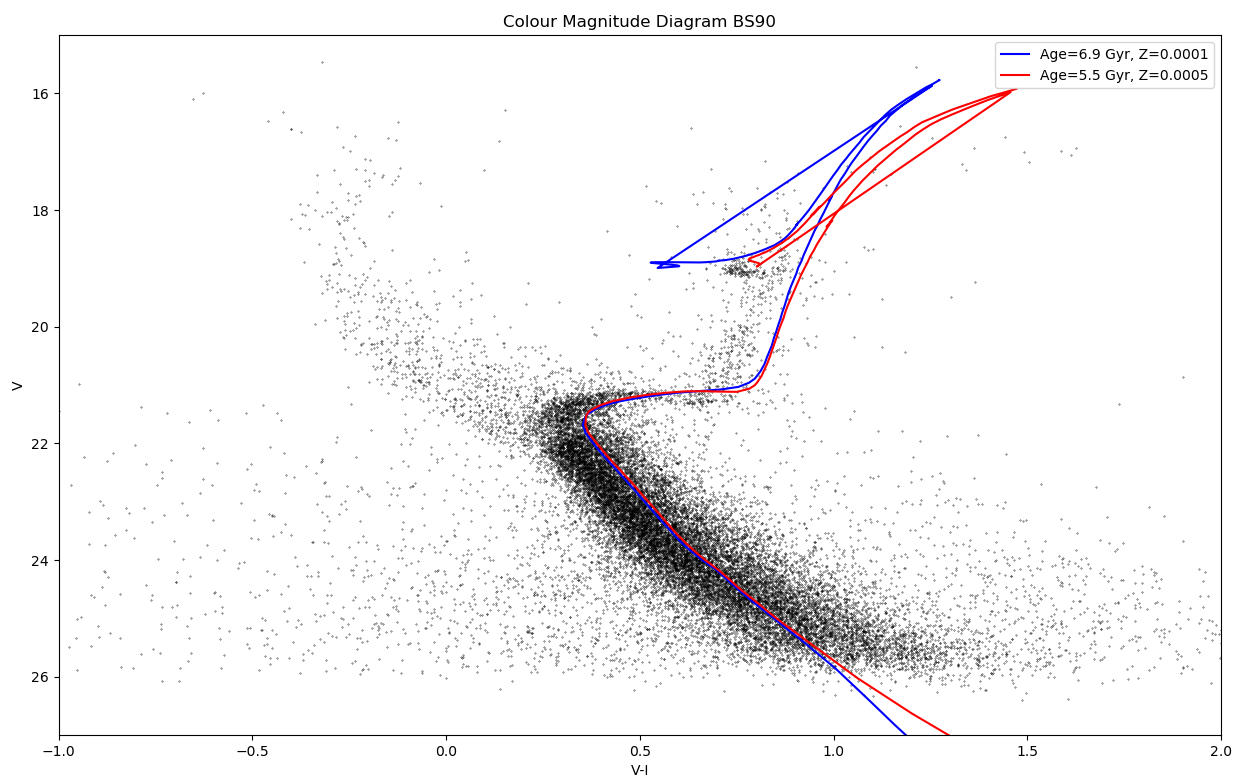
\includegraphics[width=0.8\textwidth]{report_pictures/CMDOwn.png}
	\caption{Best \textit{isochrone} fits for the CMD created with our zero point calibration}
	\label{cmd1}
\end{figure}
\vspace{3mm}\\
We used a shift of 18.8 mag for these \textit{isochrones}, which would correspond to 57.5 kpc distance to BS90. The parameter for the \textit{ischrones} we fitted is age = 6.9 Gyr with metallicity z = 0.01\% and 5.5 Gyr with z = 0.05\%. While the turn off point and the main sequence fit quite nice for the \textit{isochrones} in our CMD, the red giant branch doesn't fit very well to our CMD, pointing towards a fault in the analysis.
\vspace{2mm}\\
After researching for a while we found a paper \cite{rochau2007star} which used the same images to analyse the globular cluster BS90 and after comparing our values to theirs we noticed a big discrepancy in age and metallicity. While their distance modulus was almost the same as ours with 18.85 mag, 58.9 kpc , they approximated the age$=4.5 \pm 0.5$ Gyr and metallicity z$=0.4 \pm 0.1$\%. We then fit the values from the paper to our CMD shown in figure \ref{cmd2}. We needed to change the shift to 18.3 mag to remotely get close to a good fit, which translates to a distance of 45.7 kpc. Nonetheless it is an even worse fit then what we had beforehand.
\vspace{2mm}\\
Then we researched the origin date of the images which we found from \cite{HST_visit_report}. We then continued to determine the zeropoints calculated for the HST via the ASC zeropoint calculator \cite{HST_zeropoint}. From there we were able to determine the zeropoint for the filters to $zero_V = 25.733$ and $zero_I = 25.529$. With those new zeropoints we calculated a new cross match and plotted the CMD again, shown in figure \ref{cmd3} and this time the values of the paper fit really well for a shift of 19.0 mag, which translates to a distance of 63.1 kpc.
\begin{figure}[h]
	\begin{subfigure}{0.45\textwidth}
	\centering
	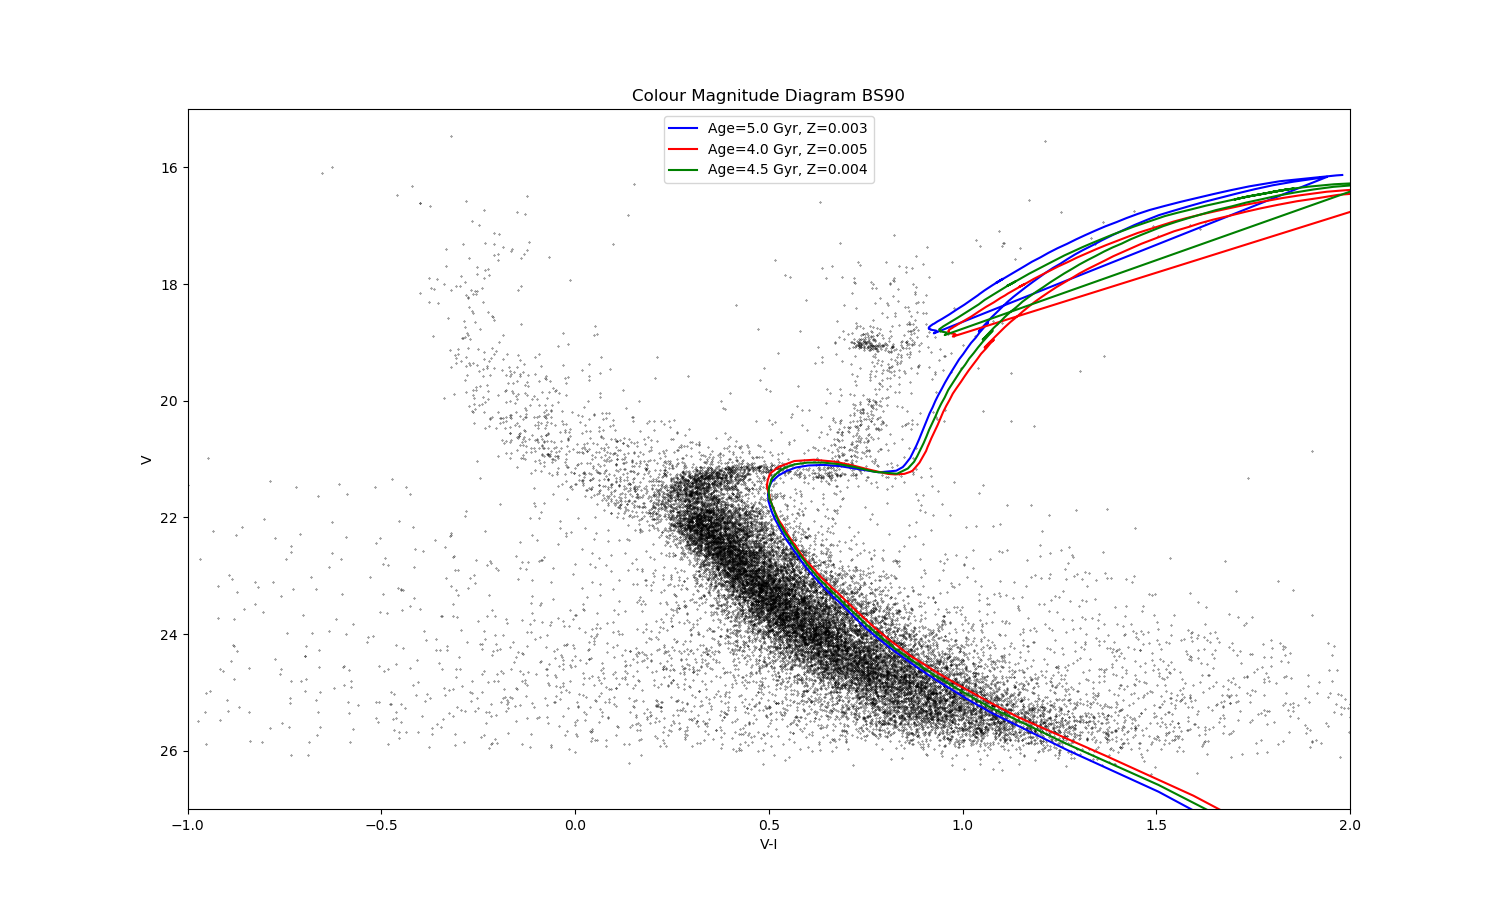
\includegraphics[width=0.95\linewidth]{report_pictures/PaperPepega.png}
	\caption{Own zeropoints}
	\label{cmd2}
	\end{subfigure}
	\begin{subfigure}{0.45\textwidth}
	\centering
	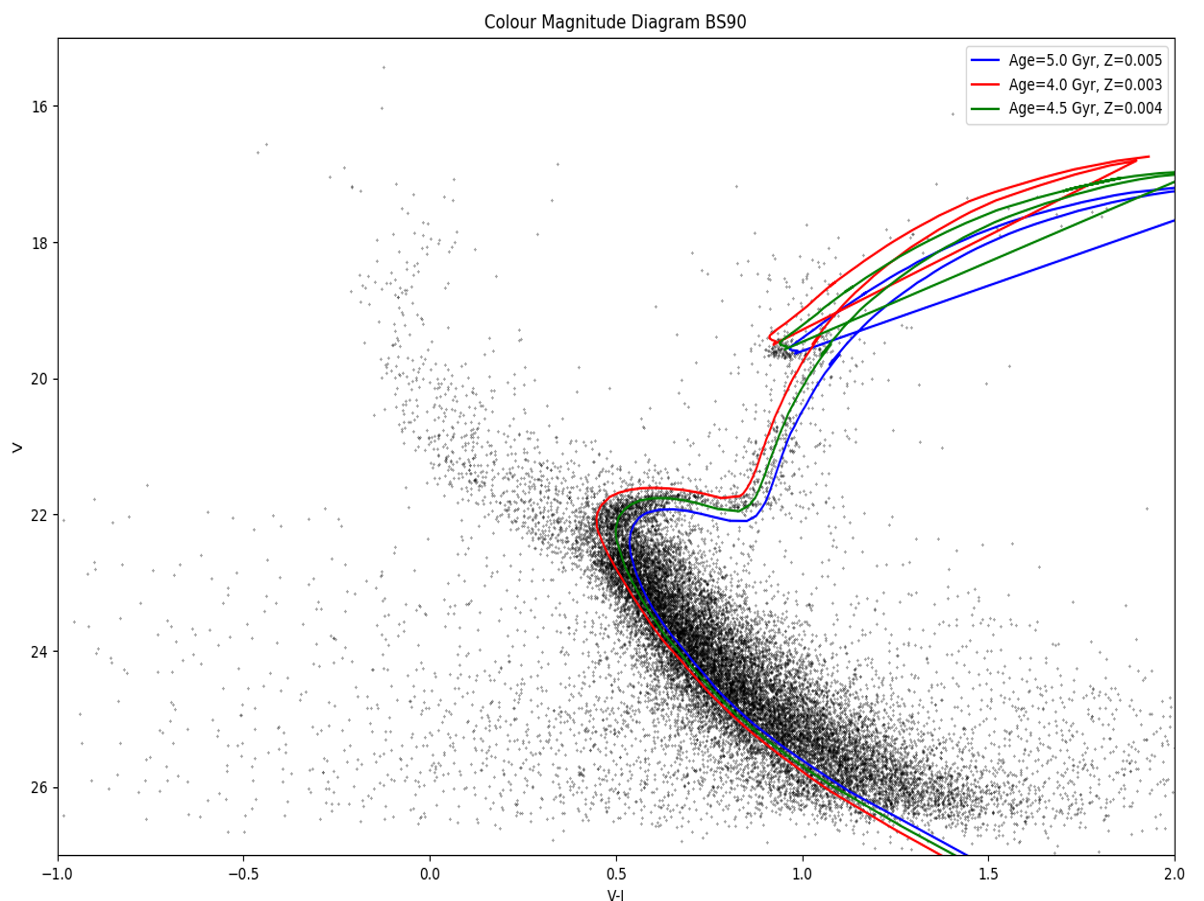
\includegraphics[width=0.95\linewidth]{report_pictures/PaperOwn.png}
	\caption{Zeropoints for calculator}
	\label{cmd3}
	\end{subfigure}
	\caption{CMDs with the age and metallicity of \cite{rochau2007star} for the \textit{isochrones}}
	\label{cmd4}
\end{figure}